\documentclass[../main.tex]{subfiles}
\begin{document}
\onlyinsubfile{
\setcounter{chapter}{0}
}
\notinsubfile{}

\begin{center}
\leavevmode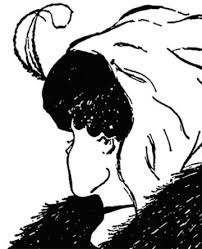
\includegraphics[width=0.5\textwidth]{./img/ovjv.png}
 \captionof{figure}{Oude vrouw jonge vrouw.
\label {fig:wbovjv}}
\end{center}

\vspace{1cm}
%\begin{center}
%\leavevmode
\begin{figure}[ht]
\def\ojfrangle{0}
\def\ojobangle{35.4}
\def\ojscale{1}
\begin{tikzpicture}%
\begin{scope}[scale=\ojscale, rotate=\ojfrangle]
  \draw[thin,gray!40] (-0.1,-0.1) grid (5,5);
  \draw[-stealth] (-0.1,0)--(5*cos{\ojobangle},0) 
        node[below, xshift=0]
        {$\alpha$}
;
  \draw[-stealth] (0,-0.1)-- (0,5*sin{\ojobangle}) 
        node[left, yshift=0]
        {$\beta$}
;
  \node[above] at (0,5) {$\ket{Young}$};
  \node[right] at (5,0) {$\ket{Old}$};
  \draw[line width=.1pt ,black] ([shift=(0:5)]0,0) arc (0:90:5);
  \draw[thick, red, -stealth](0,0)--(\ojobangle:5)
       node[label={[above, right]$\ket{\Psi}$}] (p){};
  \draw[line width=1pt,dotted] (0,5*sin{\ojobangle}) -- (p);
  \draw[line width=1pt,dotted] (p)--(5*cos{\ojobangle},0);
\end{scope}
\end{tikzpicture}
% \captionof{figure}{Teken hier je eigen toestandvectoren van jouw (W) en het klassengemiddlede (K).%
%\label{fig:wbkwadrant}}
\end{figure}
%\end{center}

\[
\ket{\Psi}=\alpha\ket{Old}+\beta\ket{Young}
\]
 
\end{document}
